\chapter{Track Laydown}
\label{chap:track-laydown}

The Method of Characteristics (MOC) has seen significant interest in the past several decades owing to the computational efficiency and flexibility of the method to model complex geometries. Several production neutronics codes utilize 2D MOC for lattice physics or full core neutronics calculations. Full core analysis using MOC has typically followed a 2D/1D approach \cite{ntracer, decart, 2d1d, CRX}. In this approach, 2D MOC is used in the radial direction while transport in the axial direction is modeled with a low order diffusion operator that uses transverse leakage to couple the radial planes. Recently, several codes has been written or extended to perform direct MOC calculations in 3D \cite{kochunas, MCI, 3D-MOC-annals}. Extending MOC to 3D comes with a wide array of challenges.

One of the areas that has been investigated recently is the development of procedures to create 3D tracks. The modular ray tracing (MRT) method developed by Filippone \cite{orig-moc-rt} has seen wide adoption in codes including MPACT \cite{mpact, kochunas}, DeCART \cite{decart}, DRAGON \cite{MCI}, CRX \cite{3D-MOC-annals}, PEACH \cite{PEACH}, and nTRACER \cite{ntracer} as a way to reduce the memory and compute time required to generate tracks for a large 3D geometry. While simple in theory, MRT requires all domains to be the same size which can lead to load imbalance issues during segmentation if the minimum repeating domain is too large. Additionally, when certain simplifications are used, the z-spacing between 3D tracks can be limited for shallow polar angles \cite{kochunas}. This results in additional memory and compute requirements that could prove burdensome when trying to produce high fidelity solutions to full core PWR problems. Studies performed on 3D MOC often use pin cell domains during the MRT segmentation process when simplified problems such as the 3D C5G7 benchmark are solved \cite{kochunas}. With the small domain sizes, the load imbalance issues are trivial. However, in real PWR problems such as the BEAVRS benchmark \cite{beavrs}, the strict pin cell structure is no longer preserved due to the presence of the grid sleeve and inter-assembly water gap. Furthermore, the presence of grid spacers, flow nozzles, and the bottom support plate result in uneven axial zone heights in the geometry. These characteristics complicate MRT and suggest a more streamlined, global approach to generating tracks might be more practical. 

In this paper, we describe the conditions required for cyclic ray tracing and present a new procedure for creating global 3D tracks that is independent of the domain decomposition scheme used. This new method, which we call 3D Global Tracking (3DGT), uses information about the 2D track cycles to perform a global fitting to ensure cyclic wrapping of 3D tracks. In order to highlight the benefits of this method, we present the number of tracks required for the MRT, simplified MRT, and 3DGT methods using anticipated parameters for a converged 3D MOC solution of a PWR core. 

\section{2D Tracking}

The Method of Characteristics is a widely used method for finding the solution of partial differential equations in which a two or three dimensional problem is approximated by solving the transport equation along constant angle tracks that traverse the geometry. While one dimensional, each track represents a particular three dimensional volume and angular subspace. The first step in setting up the MOC problem is creating tracks that span the spatial and angular space of the problem. In Fig. \ref{sample-tracks}, a sparse 2D and 3D track laydown for a homogeneous cube geometry is illustrated.

% insert picture of 2D and 3D tracks
\begin{figure}[H]
	\vspace{-0.1in}
	\centering
	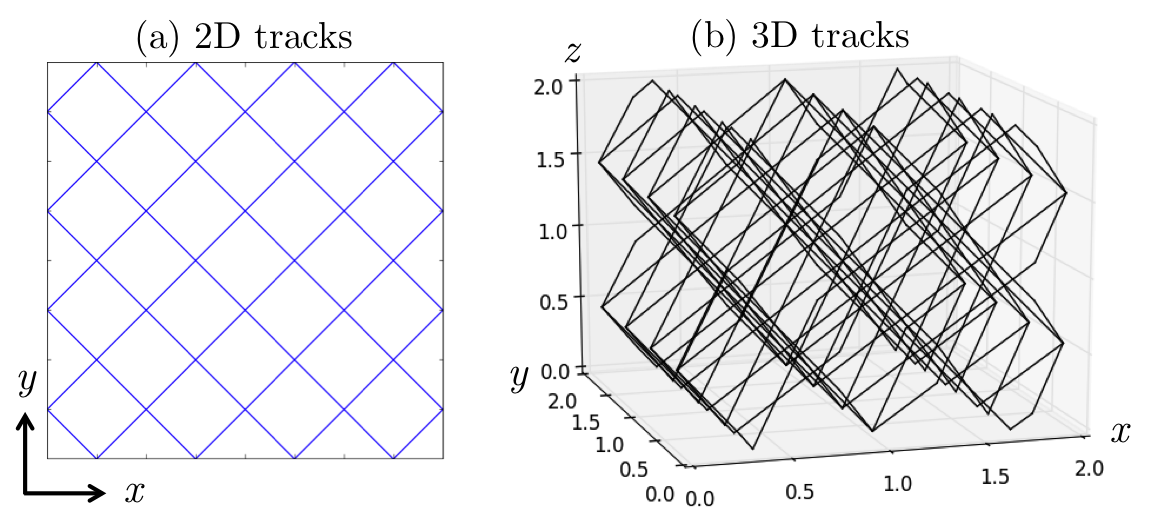
\includegraphics[width=4in]{figures/mc2015/sample-tracks-2.png}
	\caption{Pictures illustrating 2D (a) and 3D (b) tracks for a homogeneous cube geometry.}
	\label{sample-tracks}
\end{figure}

When creating the tracks, it is important to consider the boundary conditions as these determine whether the outgoing angular flux needs to be passed as the incoming flux to another track. In this study, we focus on generating tracks that are cyclic and can therefore be used for reflective or vacuum boundary conditions. While analysis of full-core problems typically involves only vacuum boundaries, it is helpful to have the option for reflective boundaries to compare the results of small-core benchmarks, such as the C5G7 benchmark, to other codes.

In our discussion, it is important that we make clear the distinction between tracks and segments (sometimes referred to as intersections). Tracks are defined to span an entire geometry or geometry subdomain and pass through region boundaries. When setting up a problem, tracks are decomposed into segments that span only a single region. Fig. \ref{tracks-vs-segments} illustrates a fine track and segment laydown for a pin cell geometry. In this study, we focus only on the track generation procedure.
%
% insert picture of fine 2D tracks and segments for a BEAVRS pin cell.
\begin{figure}[H]
	\vspace{-0.25in}
	\centering
	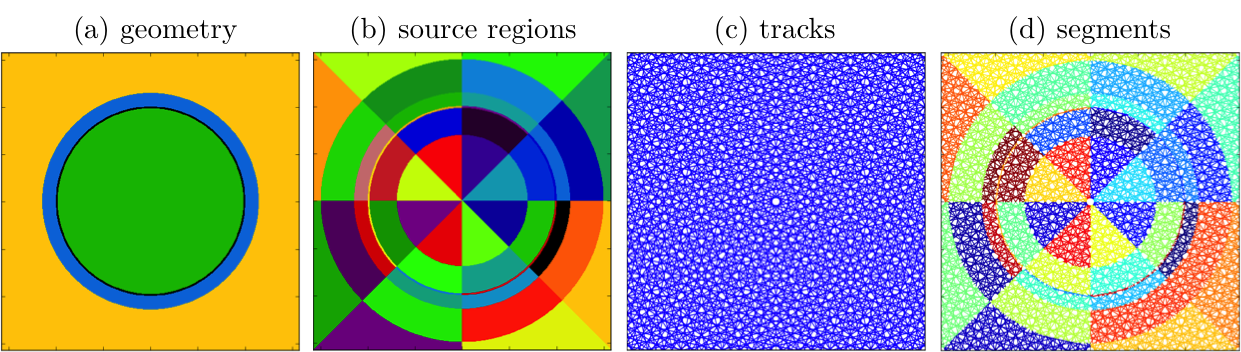
\includegraphics[width=6.5in]{figures/mc2015/tracks-vs-segments.png}
	\caption{Pictures illustrating the geometry (a), the geometry subdivided into source regions (b), a fine 2D track laydown (c), and the corresponding segment laydown colored by source region (d) for a 2D pin cell geometry containing fuel, gap, clad, and moderator materials.}
	\label{tracks-vs-segments}
	\vspace{-0.5in}
\end{figure}

Before discussing the methodology for 3D track generation, we discuss how global tracks are generated for 2D problems. Tracks for a 2D MOC problem are typically laid down using the cyclic tracking approach as illustrated in Fig. \ref{figure 3D tracks}. Users input a desired azimuthal track spacing, $\boldsymbol{\delta_\phi}$, and number of azimuthal angles, $n_{\phi}$, in 0 < $\phi$ < $2 \pi$. With this approach, azimuthal angles are created to evenly subdivide the angular space such that each azimuthal angle in 0 < $\phi$ < $\frac{\pi}{2}$ is paired with a complementary azimuthal angle,

\begin{equation}
\boldsymbol{\phi^i} = \frac{2 \pi}{n_\phi} (0.5 + i) \qquad \forall \qquad i = \Big[0,\frac{n_{\phi}}{2}\Big)
\end{equation}
%
\begin{equation}
\boldsymbol{\phi^{\frac{n_{\phi}}{2} - i - 1}} = \pi - \boldsymbol{\phi^i} \qquad \forall \qquad i= \Big[0,\frac{n_{\phi}}{4}\Big),
\end{equation} 

\noindent
where $\boldsymbol{\phi^{\frac{n_{\phi}}{2} - i - 1}}$ is the complement of angle $\boldsymbol{\phi^i}$. Other valid angular quadrature sets have also been used \cite{3D-MOC-annals}. By tracking both forward and backward along a track, the full $2 \pi$ angular space is covered as shown in Fig. \ref{figure 3D tracks} for four azimuthal angles. Tracks are laid down such that they intersect with a complementary track at the boundaries. 

% insert picture of cyclic tracking and backwards tracking
\begin{figure}[H]
	\vspace{-0.1in}
	\centering
	\includegraphics[width=4in]{figures/mc2015/fwd_bwd_tracking_2.png}
	\caption{Pictures illustrating forward (a) and backward (b) tracking for 2D MOC track laydown. The geometry width $\Delta x$, geometry height $\Delta y$, and track angles and spacing (collectively $\phi^i$, $\phi^{\frac{n_{\phi}}{2} - i - 1}$, $\delta_{\phi}^i$, $\delta_x^i$, and $\delta_y^i$) have been denoted on the pictures.}
	\label{figure 3D tracks}
\end{figure}

In order to guarantee cyclic wrapping of 2D tracks, there must be an integer number of tracks on x and y axes for a particular angle, $\boldsymbol{\phi^i}$,

\begin{equation}
\vspace{-0.1in}
\delta_x^i = \frac{\Delta x}{n_x^i} \qquad \delta_y^i = \frac{\Delta y}{n_y^i}
\label{eqn:3DGT-dx-dy}
\end{equation}

\noindent
where $n_x^i$ is the integer number of tracks along the x axis for angle $\boldsymbol{\phi^i}$. The same notation applies to the y direction. Using the input value of $\boldsymbol{\delta_{\phi}}$, the integer number of tracks along the axes for a particular angle $\boldsymbol{\phi^i}$ are computed,

\begin{equation}
%n_x^i = \ceil*{\Bigg(\frac{\Delta x \cdot \text{sin} (\boldsymbol{\phi^i})}{\boldsymbol{\delta_{\phi}}}\Bigg)} \qquad n_y^i = \ceil*{\Bigg(\frac{\Delta y \cdot \text{cos} (\boldsymbol{\phi^i})}{\boldsymbol{\delta_{\phi}}}\Bigg)}
FIXME
\label{eqn:3DGT-nx-ny}
\end{equation}

\noindent
where the ceiling is taken to ensure at least one track intersects with each axis. The azimuthal angle is then corrected,

\begin{equation}
\phi^i = \text{tan}^{-1} \bigg(\frac{\delta_y^i}{\delta_x^i}\bigg)
\label{eqn:azi-correct}
\end{equation}

\noindent
where $\phi_i$ is used to denote the corrected azimuthal angle. Using the corrected azimuthal angle, the azimuthal track spacing for each angle is also corrected,

\begin{equation}
\delta_{\phi}^i = \delta_x^i \cdot \text{sin} (\phi^i)
\label{eqn:azi-space-correct}
\end{equation}

\noindent
where $\delta_{\phi}^i$ is used to denote the corrected azimuthal track spacing. Using the corrected values, $\phi^i$ and $\delta_{\phi}^i$, the 2D tracks are laid down on the geometry. 

\section{3D tracking}

\subsection{Requirements for Cyclic Track Laydown in 3D}

In generating 3D tracks, we assume that 3D tracks are laid down as z-stacked arrays of tracks that project down onto the 2D track layout. Before discussing the conditions required to generate cyclic tracks in 3D, we need to understand the concept of a reflective track cycle. Fig. \ref{figure 2} decomposes a sample 2D geometry into 2D reflective track cycles with $T_{R,k}^{i}$ denoting the $k^{th}$ reflective track cycle for azimuthal angle $\phi^i$. 

% insert picture
\begin{figure}[h]
	\vspace{-0.05in}
	\centering
	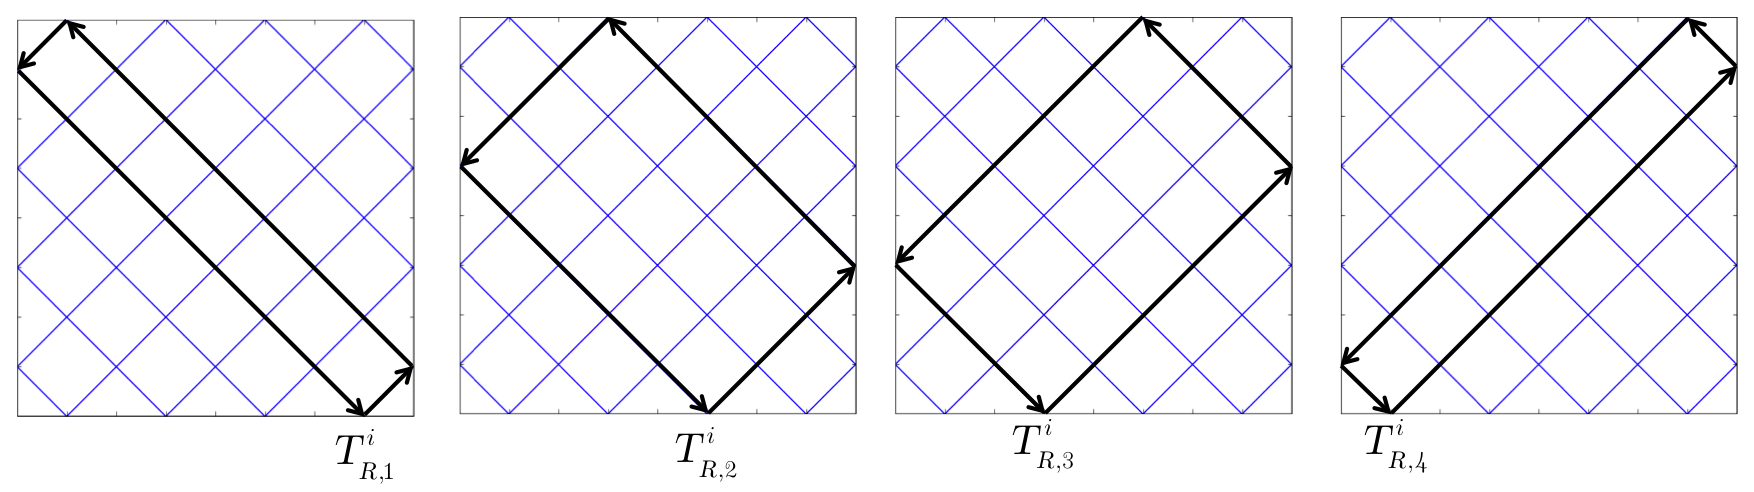
\includegraphics[width=6.5in]{figures/mc2015/reflective-track-cycles-3.png}
	\caption{Each plot highlights one of the 2D track cycles contained in a sample geometry. The reflective track cycles are labeled with $T_{R,k}^{i}$ denoting the $k^{th}$ track cycle for azimuthal angle $\phi^i$.}
	\label{figure 2}
\end{figure}

\noindent
To generate 3D tracks, users input a desired polar track spacing, $\boldsymbol{\delta_\theta}$, and number of polar angles, $n_{\theta}$, in 0 < $\theta$ < $\pi$ in addition to the parameters required to generate 2D tracks. With this approach, polar angles are created to evenly subdivide the angular space such that each polar angle in $0 < \theta < \frac{\pi}{2}$ is paired with a complementary polar angle,

\begin{equation}
\boldsymbol{\theta^{i,j}} = \frac{\pi}{n_{\theta}} \cdot (0.5 + j) \qquad \forall \qquad j = \Big[0,\frac{n_{\theta}}{2}\Big)
\end{equation}

\begin{equation}
\boldsymbol{\theta^{i,n_{\theta} - j - 1}} = \pi - \boldsymbol{\theta^{i,j}} \qquad \forall \qquad j= \Big[0,\frac{n_{\theta}}{2}\Big),
\end{equation} 

\noindent
where $\boldsymbol{\theta^{i,n_{\theta} - j - 1}}$ is the complement of angle $\boldsymbol{\theta^{i,j}}$. Note that the polar angles are initially defined to be independent of azimuthal angle index, $i$. Later, we use the azimuthal angle to correct the polar angle to ensure the tracks are cyclic. Following the same notation used to describe the azimuthal angles, the corrected polar angles will be denoted by $\theta^{i,j}$. By tracking both forward and backward along a track, the full $4 \pi$ angular space can be covered as shown in Fig. \ref{sample-tracks} for four azimuthal and two polar angles.

Tracks are laid down such that they intersect with a complementary track at the boundaries. Selecting an arbitrary cycle, $T_{R,k}^{i}$, we follow a set of 3D tracks as they complete one 2D cycle. Fig. \ref{figure 3} highlights a particular 2D track cycle and a set of 3D tracks projected along that cycle.

% insert picture
\begin{figure}[h]
	\vspace{-0.1in}
	\centering
	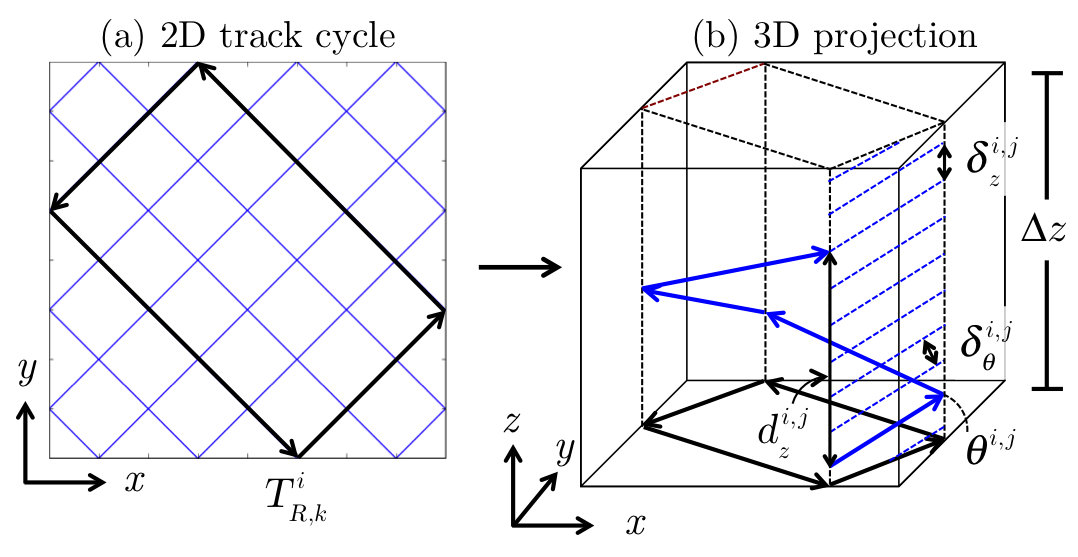
\includegraphics[width=4.5in]{figures/mc2015/track_cycles_3.png}
	\caption{Illustration of an arbitrary 2D track cycle (a), $T_{R,k}^{i}$, and a set of 3D tracks projected along the 2D track cycle (b).}
	\label{figure 3}
\end{figure}

\noindent
To guarantee cyclic track wrapping of the 3D tracks, two conditions must be met:

\begin{enumerate}
	\item For each azimuthal angle, $\phi^i$, polar angle, $\theta^{i,j}$, and 2D track cycle, $T_{R,k}^{i}$, the distance between the beginning and end of a 3D track projection along a 2D track cycle must be an integer number of track spacings.
	\item For each azimuthal angle, $\phi^i$, and polar angle, $\theta^{i,j}$, there must be an integer number of track spacings along the z axis over the depth of geometry, $\Delta z$.
\end{enumerate}

The first condition guarantees that a 3D track cycle wraps back onto another 3D track when the 2D reflective cycle is completed. The second condition guarantees that a 3D track cycle that contains a reflection off a top or bottom surface still reflects into an existing 3D track when the 2D cycle is completed. In the next two sections, we show how both the 3DGT and MRT methods comply with these conditions and what additional assumptions they make.

\subsection{The 3D Global Tracking Method}

The 3DGT method uses the conditions stated in the previous section for 3D cyclic ray tracing to generate tracks for a rectangular geometry independent of any domain decomposition scheme. After the 2D track information has been generated, the 3D track information can be computed using the requirements for 3D cyclic global ray tracing. First, we note that all 2D track cycles for a particular azimuthal angle index, $i$, have the same cycle length that can be computed,

\begin{equation}
L_R^i = \text{lcm}\bigg( 2 \cdot n_x^i,  \frac{2 \cdot \Delta y}{\text{tan} (\phi^i) \cdot \delta_x^i} \bigg) \cdot \frac{\delta_x^i}{\text{cos} (\phi^i)},
\label{eqn:refl-cycle-len}
\end{equation}

\noindent
where lcm is the least common multiple. There are several ways in which the 3D track information can be found given a user specified polar spacing and number of polar angles. The method we use below is well suited towards minimizing the correction to the desired polar angles while allowing the polar track spacing to change significantly. Using the reflective cycle length for each azimuthal angle, the integer number of track spacings between the beginning and end of a set of 3D tracks after one complete 2D cycle can be computed,

\begin{equation}
%n_l^{i} = \ceil*{L_R^i \cdot \text{cot} (\boldsymbol{\theta^{i,j}}) \cdot \frac{\text{sin} (\boldsymbol{\theta^{i,j})}}{\boldsymbol{\delta_{\theta}}}},
FIXME
\label{eqn:3DGT-nl}
\end{equation}

\noindent
where $L_R^i \cdot \text{cot} (\boldsymbol{\theta^{i,j}})$ is the z distance between the start and end of the set of 3D tracks, $\frac{\text{sin} (\boldsymbol{\theta^{i,j}})}{\boldsymbol{\delta_{\theta}}}$ is the z distance between tracks, and the subscript $l$ is used to signify that $n_l^i$ is measured along the direction of a track cycle. Next, the number of track spacings along the z axis needs to be set to an integer number. The number of tracks on the z axis can be found by considering the relation between the number of track spacings in the z direction and the spacing along the length of the 2D track.

\begin{equation}
\text{tan} (\theta^{i,j}) = \frac{\delta_L^i}{\delta_z^{i,j}} = \frac{L_R^i}{n_l^i} \cdot \frac{n_z^{i,j}}{\Delta z}
\end{equation}

\noindent
Rearranging and inserting our approximation for the polar angle, $\boldsymbol{\theta^{i,j}}$, this equation gives us an expression for the number of tracks on the z axis,

\begin{equation}
%n_z^{i,j} = \ceil*{\frac{\Delta z \cdot n_l^i \cdot \text{tan} (\boldsymbol{\theta^{i,j}})}{L_R^i}},
FIXME
\label{eqn:3DGT-nz}
\end{equation}

\noindent
where we take the ceiling to ensure at least one track crossing on the z axis. The z-spacing between 3D tracks is shown in Eq. \ref{eqn:3DGT-delta-z}.

\begin{equation}
\delta_z^{i,j} = \frac{\Delta z}{n_z^{i,j}}
\label{eqn:3DGT-delta-z}
\end{equation}

\noindent
Using the 2D cycle length and number of track crossings on the z axis and along the length of the 2D cycle, the polar angle can be corrected using Eq. \ref{eqn:3DGT-theta-correct}.

\begin{equation}
\theta^{i,j} = \text{tan}^{-1} \bigg( \frac{L_R^i}{n_l^i \cdot \delta_z^{i,j}}\bigg)
\label{eqn:3DGT-theta-correct}
\end{equation}

\noindent
Similarly, the polar track spacing is corrected using Eq. \ref{eqn:3DGT-dtheta-correct}.

\begin{equation}
\delta_\theta^{i,j} = \delta_z^{i,j} \cdot \text{sin} (\theta^{i,j})
\label{eqn:3DGT-dtheta-correct}
\end{equation}

\noindent
In summary, the algorithm for generating tracks with the 3DGT method is described by Alg. \ref{alg:3DGT}.

\begin{algorithm*}[!h]
	\caption{3D track generation using the 3D Global Tracking Method}
	\label{alg:3DGT}
	%\begin{algorithmic}
	%	\STATE User specifies $n_{\phi}$, $\boldsymbol{\delta_{\phi}}$, $n_{\theta}$, and $\boldsymbol{\delta_{\theta}}$. \hspace{\fill}
%		\FORALL[Loop over azimuthal angles]{$i \in I$}
%		\STATE Compute the \# of tracks in x and y for $\boldsymbol{\phi^i}$, $n_x^i$ and $n_y^i$, and distance between tracks in x and y, $\delta_x^i$ and $\delta_y^i$ (Eqs. \ref{eqn:3DGT-dx-dy} and \ref{eqn:3DGT-nx-ny}). \hspace{\fill}
		
%		\STATE Correct the azimuthal angle and azimuthal track spacing, $\phi^i$ and $\delta_{\phi}^i$ (Eqs. \ref{eqn:azi-correct} and \ref{eqn:azi-space-correct}).
		
%		\STATE Compute the length of the 2D reflective track cycles, $L_R^{i}$ (Eqs. \ref{eqn:refl-cycle-len}).
		
%		\FORALL[Loop over polar angles]{$j \in J$}
		
%		\STATE Compute the \# of track spacings after one complete 2D cycle, $n_l^{i,j}$ (Eq. \ref{eqn:3DGT-nl}).
		
%		\STATE Compute the \# of tracks on the z axis, $n_z^{i,j}$ (Eq. \ref{eqn:3DGT-nz}).
		
%		\STATE Compute the z distance between 3D tracks, $\delta_z^{i,j}$ (Eq. \ref{eqn:3DGT-delta-z}).
		
%		\STATE Correct the polar angle, $\theta^{i,j}$ (Eq. \ref{eqn:3DGT-theta-correct}).
		
%		\STATE Correct the polar track spacing, $\delta_{\theta}^{i,j}$ (Eq. \ref{eqn:3DGT-dtheta-correct}).
		
%		\ENDFOR
%		\ENDFOR
%	\end{algorithmic}
FIXME
\end{algorithm*}

\subsection{The Modular Ray Tracing Method}

Modular ray tracing relies on the principle that a geometry can be uniformly decomposed into a series of rectangular cuboids of equal size. Typically, the decomposition procedure is performed such that many of the cuboids have the same underlying geometry and therefore contain the same segment structure. This allows an identical set of tracks to be laid down on each domain and segmentation only performed on each unique domain type. Therefore, we only present the track generation procedure for a single domain. 

The MRT method uses a procedure similar to that used in the 3DGT method for track generation. For a domain, the number of tracks and spacing between tracks in x and y are described in Eq. \ref{eqn:mrt-nx-ny} and Eq. \ref{eqn:mrt-dx-dy}, respectively,

\begin{equation}
%n_x^i = \ceil*{\Bigg(\frac{\Delta x \cdot \text{sin} (\boldsymbol{\phi^i})}{D_x \cdot \boldsymbol{\delta_{\phi}}}\Bigg)} \qquad n_y^i = \ceil*{\Bigg(\frac{\Delta y \cdot \text{cos} (\boldsymbol{\phi^i})}{D_y \cdot \boldsymbol{\delta_{\phi}}}\Bigg)}
FIXME
\label{eqn:mrt-nx-ny}
\end{equation}

\begin{equation}
\delta_x^i = \frac{\Delta x}{D_x \cdot n_x^i} \qquad \delta_y^i = \frac{\Delta y}{D_y \cdot n_y^i},
\label{eqn:mrt-dx-dy}
\end{equation}

\noindent
where $D_x$ and $D_y$ are the integer number of domains in the x and y directions, respectively. This guarantees that an integer number of tracks lie along the x and y boundaries of each domain cell and that tracks on one surface line up with adjoining tracks in the neighbor domain cell. 

When generating tracks using the MRT method, it is important to remember that a track crossing a domain interface needs to connect with another track on the neighboring domain. As we follow a series of tracks across the geometry, we notice that the series of tracks is periodic. A periodic track cycle is defined to be the series of domain tracks that repeats when a global track traverses a geometry. Fig. \ref{periodic cycles} shows the periodic track cycles for one azimuthal angle in our sample geometry when it is split into four domains.

% insert picture
\begin{figure}[h]
	\centering
	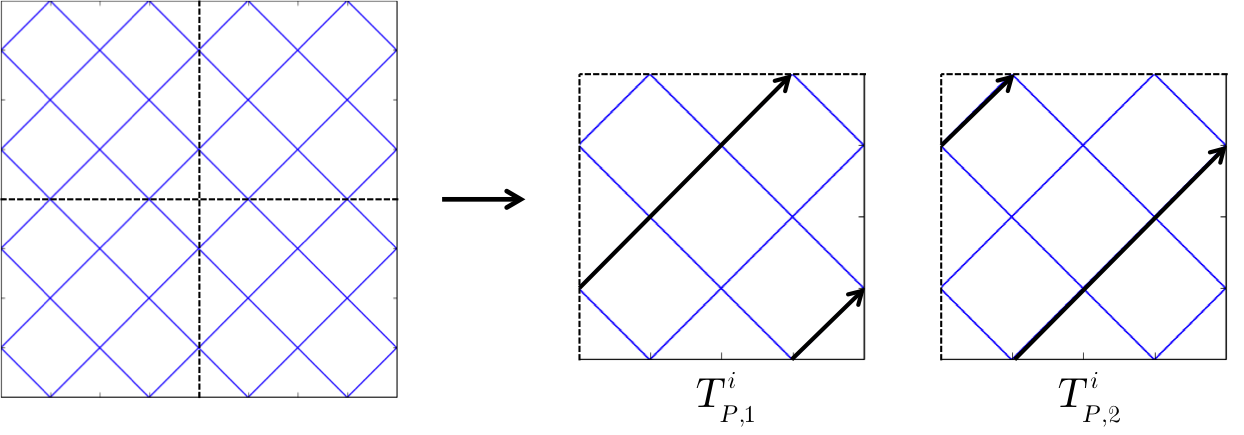
\includegraphics[width=5in]{figures/mc2015/2d_periodic_track_cycles_2.png}
	\caption{Each plot highlights one of the 2D periodic track cycles contained in a sample geometry split into four domains of equal size. The track cycles are labeled with $T_{P,k}^i$ denoting the $k^{th}$ periodic track cycle for azimuthal angle $\phi^i$.}
	\label{periodic cycles}
\end{figure}

We can define the length of the periodic track cycles for each azimuthal angle to be $L_P^{i}$. For the MRT method, the periodic 2D track cycles for a particular azimuthal angle, $i$, have the same cycle length computed in Eq. \ref{eqn:period-cycle-len}.

\begin{equation}
L_P^i = \text{lcm} \bigg( n_x^i,  \frac{\Delta y}{D_y \cdot \text{tan} (\phi^i) \cdot \delta_x^i} \bigg) \cdot \frac{\delta_x^i}{\text{cos} (\phi^i)}
\label{eqn:period-cycle-len}
\end{equation}


\noindent
The procedure to find the corrected polar track spacing and corrected polar angles is identical to the procedure used in the 3DGT method, except that $L_R^i$ is replaced with $L_P^i$ and $\Delta z$ is replaced with $\frac{\Delta z}{D_z}$.

The procedure for identifying the periodic track cycles and finding the start and end points for all tracks using the MRT and 3DGT methods can seem a bit tedious, so others have simplified the MRT method by noticing that the lengths of all 2D tracks are an integer multiple of the shortest 2D track \cite{kochunas}. For example, the length of the first three 2D tracks, $t_1^i$, $t_2^i$, and $t_3^i$, for azimuthal angle $\phi^i$ are shown in Eqs. \ref{eqn:short-track}, \ref{eqn:short-track-2}, and \ref{eqn:short-track-3}.

\begin{equation}
l_1^i = \sqrt{\bigg[\frac{\delta_x^i}{2}\bigg]^2 + \bigg[\frac{\delta_y^i}{2}\bigg]^2} = \frac{1}{2} \sqrt{(\delta_x^i)^2 + (\delta_y^i)^2}
\label{eqn:short-track}
\end{equation}

\begin{equation}
l_2^i = \sqrt{\bigg[\frac{3 \delta_x^i}{2}\bigg]^2 + \bigg[\frac{3 \delta_y^i}{2}\bigg]^2} = \frac{3}{2} \sqrt{(\delta_x^i)^2 + (\delta_y^i)^2} = 3 l_1^i
\label{eqn:short-track-2}
\end{equation}

\begin{equation}
l_3^i = \sqrt{\bigg[\frac{5 \delta_x^i}{2}\bigg]^2 + \bigg[\frac{5 \delta_y^i}{2}\bigg]^2} = \frac{5}{2} \sqrt{(\delta_x^i)^2 + (\delta_y^i)^2} = 5 l_1^i
\label{eqn:short-track-3}
\end{equation}

Since the length of all 2D tracks is an integer number of lengths of the first track, $l_1^i$, any valid track laydown for the first track is also valid for all other tracks. Therefore, we can set the cycle length for an azimuthal angle, $L_P^i$, to the length of the shortest track, $l_1^i$. The algorithm for generating tracks for the MRT and simplified MRT (s-MRT) method can be described by Alg. \ref{alg:MRT}. 

\begin{algorithm*}[!h]
	\caption{3D track generation using the Modular Ray Tracing Method}
	\label{alg:MRT}
	FIXME
	%\begin{algorithmic}
	%	\STATE User specifies $n_{\phi}$, $\boldsymbol{\delta_{\phi}}$, $n_{\theta}$, $\boldsymbol{\delta_{\theta}}$, $D_x$, $D_y$, and $D_z$. \hspace{\fill}
	%	\FORALL[Loop over azimuthal angles]{$i \in I$}
	%	\STATE Compute the \# of tracks in x and y for $\boldsymbol{\phi^i}$, $n_x^i$ and $n_y^i$, and distance between tracks in x and y, $\delta_x^i$ and $\delta_y^i$ (Eq. \ref{eqn:mrt-nx-ny} and \ref{eqn:mrt-dx-dy}). \hspace{\fill}
		
	%	\STATE Correct the azimuthal angle and azimuthal track spacing, $\phi^i$ and $\delta_{\phi}^i$ (Eqs. \ref{eqn:3DGT-dx-dy} and \ref{eqn:3DGT-nx-ny}).
		
	%	\IF{MRT}  
	%	\STATE Compute the length of the 2D periodic track cycles, $L_P^{i}$ (Eq. \ref{eqn:period-cycle-len}).
		
	%	\ELSE 
	%	\STATE Compute the length of the shortest track, $l_1^i$ (Eq. \ref{eqn:short-track}). 
		
	%	\ENDIF
		
	%	\FORALL[Loop over polar angles]{$j \in J$}
		
	%	\STATE Compute the \# of track spacings after one complete 2D cycle, $n_l^{i,j}$.
		
	%	\begin{equation}
	%	n_l^{i} = \ceil*{L_P^i \cdot \text{cot} (\boldsymbol{\theta^{i,j}}) \cdot \frac{\text{sin} (\boldsymbol{\theta^{i,j}})}{\boldsymbol{\delta_{\theta}}}}
	%	\nonumber
	%	\end{equation}
		
	%	\STATE Compute the \# of tracks on the z axis, $n_z^{i,j}$.
		
	%	\begin{equation}
	%	n_z^{i,j} = \ceil*{\frac{\Delta z \cdot n_l^i \cdot \text{tan} (\boldsymbol{\theta^{i,j}})}{D_z \cdot L_P^i}}
	%	\nonumber
	%	\end{equation}
		
	%	\STATE Compute the z-distance between 3D tracks, $\delta_z^{i,j}$.
		
	%	\begin{equation}
	%	\delta_z^{i,j} = \frac{\Delta z}{D_z \cdot n_z^{i,j}}
	%	\nonumber
	%	\end{equation}
		
	%	\STATE Correct the polar angle, $\theta^{i,j}$.
		
	%	\begin{equation}
	%	\theta^{i,j} = \text{tan}^{-1} \bigg( \frac{L_P^i}{n_l^i \cdot \delta_z^{i,j}}\bigg)
	%	\nonumber
	%	\end{equation}
		
	%	\STATE Correct the polar track spacing, $\delta_{\theta}^{i,j}$ (Eq. \ref{eqn:3DGT-dtheta-correct}).
		
	%	\ENDFOR
	%	\ENDFOR
	%\end{algorithmic}
\end{algorithm*}

It is important to note that the track generation procedure described in Alg. \ref{alg:MRT} favors correcting the polar track spacing over correcting the polar angle. Alternative algorithms could easily be designed to favor correcting the polar angle over the polar track spacing, but it is expected that correcting the polar track spacing is a more conservative procedure and this is in line with previous work on MRT \cite{kochunas}. When the periodic cycle length is small relative to the desired polar track spacing, the correction to the polar track spacing can be very large. This has significant implications for the s-MRT method where the periodic cycle length is always on the order of the azimuthal track spacing. For instance, if we consider the case of a shallow polar angle ($\boldsymbol{\theta}$ near $\frac{\pi}{2}$) where $\boldsymbol{\phi} = \frac{\pi}{4}$, $\boldsymbol{\theta} = 0.9 \cdot \frac{\pi}{2}$, $\boldsymbol{\delta_\phi} = 0.05$, and $\boldsymbol{\delta_\theta} = 0.25$ for an infinitely tall domain, the s-MRT method produces a corrected polar track spacing of $\delta_\theta^{i,j} \approx 0.0079$. This increases the number of tracks for this direction by a factor of $\sim$32 over the ideal case and in Sec. \ref{implications} we discuss the memory implications of this characteristic in more detail. 

Additionally, others have claimed that the MRT method must store all tracks in the unit sphere while the s-MRT method only requires tracks in half of the unit sphere \cite{kochunas}. Our algorithm for generating tracks using the MRT and s-MRT methods (Alg. \ref{alg:MRT}) satisfies the criteria for cyclic tracking and in practice we have been able to produce cyclic track laydowns for the MRT method that require storage of tracks over only half the unit sphere. It is suspected that the previous work did not consider the track cycles as a unit and instead generated the z-stacked arrays of 3D tracks independent of other tracks in the cycle.

%%%%%%%%%%%%%%%%%%%%%%%%%%%%%%%%%%%%%%%%%%%%%%%%%%%%%%%%%%%%%%%%%%%%%
\section{Implications for 3D MOC}
\label{implications}

As a rough approximation, the required parameters to converge a full-core problem might be similar to those presented in Table~\ref{tab:full_core_reqs}. With the 3DGT method, these parameters lead to the generation of $5.66 \times 10^9$ tracks when no memory decomposition scheme is used. With this many tracks, the storage of the two 100-group angular flux vectors for each track with single precision would require 4.53 TB. This is much larger than the memory limit of current machines. For instance, the on-node memory of BlueGene/Q is constrained to 16 GB/node \cite{BGQ}.

\begin{table}[h]
	\centering
	\caption{Anticipated parameters for a converged 3D MOC solution of a PWR core.}
	\begin{tabular}{cc}
		\toprule
		\textbf{Parameter} & \textbf{Dimension} \\
		\midrule
		Height (z)                 & 455.444 cm \\
		Width (x and y)            & 365.56188 cm*\\
		Radial ray spacing         & 0.05 cm \\
		Axial ray spacing          & 0.25 cm \\
		Number of azimuthal angles & 64 \\
		Number of polar angles     & 10 \\
		\bottomrule
		\multicolumn{2}{l}{*Width assumed to be 17 assemblies in each direction.}\\
		\bottomrule
	\end{tabular}
	\label{tab:full_core_reqs}
\end{table}

For any MOC implementation, iterations are performed in which the Boltzmann neutron transport equation is solved for every characteristic track. Therefore, the computational time associated with solving any problem directly scales with the number of tracks \cite{kochunas}. In addition, the on-node memory constraints are often dominated by the storage of boundary angular fluxes for each track \cite{gunow}. The number of tracks generated using the s-MRT, MRT, and 3DGT methods using the parameters in Table~\ref{tab:full_core_reqs} is presented in Table~\ref{tab:track_laydown_comparison}. 

\begin{table}[h]
	\centering
	\caption{Number of tracks generated using the three track generation methods applied to the parameters in Table~\ref{tab:full_core_reqs}.}
	\begin{tabular}{cc}
		\toprule
		\textbf{Method} & \textbf{Number of tracks generated} \\
		\midrule
		s-MRT & $4.74 \times 10^{10}$ \\
		MRT & $5.70 \times 10^9$ \\
		3DGT & $5.66 \times 10^9$ \\
		\bottomrule
	\end{tabular}
	\label{tab:track_laydown_comparison}
\end{table}

Previous work has often used only one track spacing for both the desired azimuthal and polar track spacing \cite{kochunas, mpact}. However, due to the success of 2D/1D methods \cite{2d1d}, we anticipate that the required axial spacing will be far more coarse than the radial spacing. Fig. \ref{fig:tracks-comp} shows the number of tracks versus the ratio of desired polar to azimuthal track spacing for the parameters in Table~\ref{tab:full_core_reqs}. Both the MRT and 3DGT methods do not require large corrections on the polar track spacing due to the relatively large length of the cycle compared with the azimuthal spacing. With equal azimuthal and polar track spacing, the s-MRT method only requires $\sim$2.0 times more tracks than the 3DGT and MRT methods while for the expected parameters, the s-MRT method requires $\sim$8.4 times more tracks. This illustrates the inflexibility of the s-MRT method when applied to common reactor problems in which the radial complexity is much greater than the axial complexity and suggests that the s-MRT method should be avoided.

\begin{figure}[h]
	\centering
	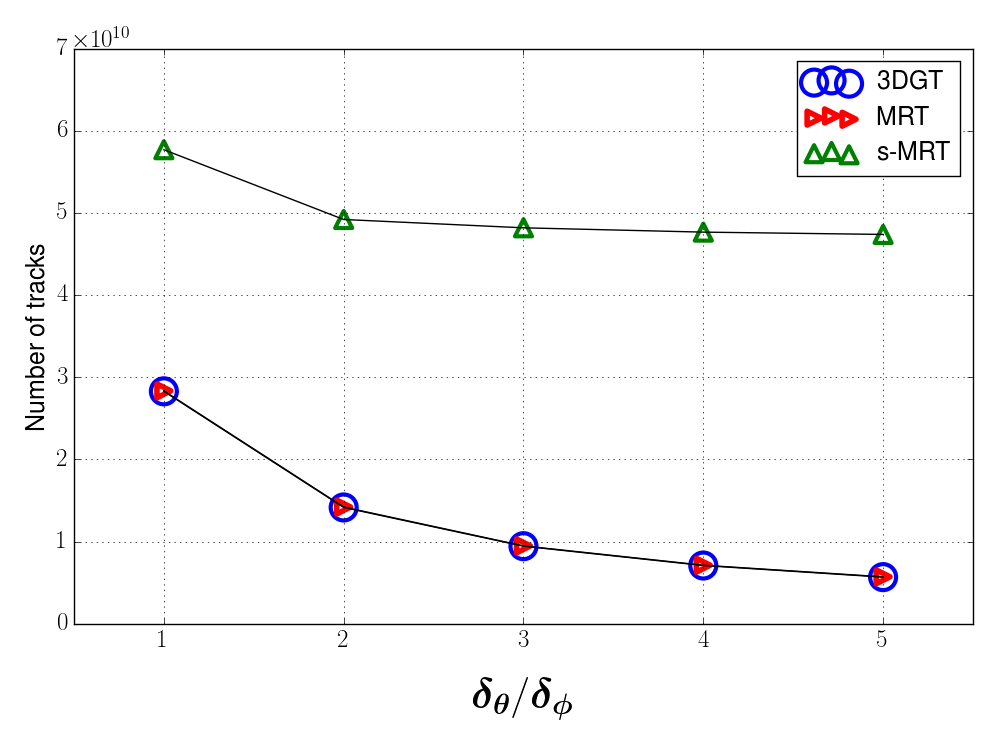
\includegraphics[width=4in]{figures/mc2015/track_comparison_2.png}
	\caption{Plot of the number of tracks versus the track polar spacing, $\boldsymbol{\delta_\theta}$, divided by the track azimuthal spacing, $\boldsymbol{\delta_\phi}$, for the specifications described in \ref{tab:full_core_reqs}. In order to change the ratio of desired polar to azimuthal spacing, the polar track spacing was modified while the desired azimuthal spacing was held constant at 0.05 cm.}
	\label{fig:tracks-comp}
\end{figure}

Incorporating a domain decomposition scheme will only increase the memory requirements further. For the 3D MOC problem presented in Table~\ref{tab:full_core_reqs}, we have assessed the memory requirements for two domain decomposition schemes with a variety of input parameters and presented the results in Table~\ref{tab:dom_dec_reqs}. The increase in storage requirements for the s-MRT method is due almost entirely to the increase in the $\boldsymbol{\delta_{\theta}}/\boldsymbol{\delta_{\phi}}$ ratio and not to the domain decomposition scheme. Reducing the number of polar angles did not have a large effect on the ratio of storage required by the s-MRT method to the storage required by the MRT and 3DGT methods either. At this point, it is unclear what the track spacing and number of azimuthal and polar angles will be to converge a full-core problem. The storage requirements for many cases in Table~\ref{tab:dom_dec_reqs} are close to or above the on-node storage of BlueGene/Q and the storage for the scalar fluxes and material cross sections has not even been taken into consideration. New machines will likely have different characteristics and it will be important to have a method this both minimizes the memory requirements and is flexible to different domain sizes.  

\begin{table}[h]
	\centering
	\caption{Number of tracks and memory requirements for full core PWR problem using quarter assembly geometry, assembly-wise domain decomposition, 64 azimuthal angles, and 0.05 cm azimuthal ray spacing.}
	\begin{tabular}{cccccccc}
		\toprule
		\textbf{Method} & \textbf{Domains ($x$,$y$,$z$)} & \textbf{$n_\theta$} & \textbf{$\boldsymbol{\delta_\theta}$ (cm)} & $\frac{\textbf{tracks}}{\textbf{domain}}$ & $\frac{\textbf{memory}}{\textbf{domain}}$ \textbf{(GB)} \\
		\midrule
		3DGT  &            &    &      & $8.65 \times 10^{6}$ & 13.8 \\
		MRT   & (17,17,21) & 10 & 0.25 & $8.71 \times 10^{6}$ & 13.9 \\
		s-MRT &            &    &      & $7.00 \times 10^{7}$ & 112.1 \\ \hline
		3DGT  &            &    &      & $4.32 \times 10^{7}$ & 69.2 \\
		MRT   & (17,17,21) & 10 & 0.05 & $4.33 \times 10^{7}$ & 69.3 \\
		s-MRT &            &    &      & $8.64 \times 10^{7}$ & 138.2 \\ \hline
		3DGT  &            &    &      & $2.16 \times 10^{6}$ & 3.5 \\
		MRT   & (34,34,42) & 10 & 0.25 & $2.18 \times 10^{6}$ & 3.5 \\
		s-MRT &            &    &      & $1.76 \times 10^{7}$ & 28.2 \\ \hline
		3DGT  &            &    &      & $1.08 \times 10^{7}$ & 17.3 \\
		MRT   & (34,34,42) & 10 & 0.05 & $1.09 \times 10^{7}$ & 17.4 \\ 
		s-MRT &            &    &      & $2.17 \times 10^{7}$ & 34.7 \\ \hline
		3DGT  &            &    &      & $8.65 \times 10^{6}$ & 8.4 \\
		MRT   & (17,17,21) & 6  & 0.25 & $8.71 \times 10^{6}$ & 8.4 \\
		s-MRT &            &    &      & $7.00 \times 10^{7}$ & 59.4 \\ \hline
		3DGT  &            &    &      & $4.32 \times 10^{7}$ & 41.8 \\
		MRT   & (17,17,21) & 6  & 0.05 & $4.33 \times 10^{7}$ & 41.9 \\
		s-MRT &            &    &      & $8.64 \times 10^{7}$ & 75.7 \\ \hline
		3DGT  &            &    &      & $2.16 \times 10^{6}$ & 2.1 \\
		MRT   & (34,34,42) & 6  & 0.25 & $2.18 \times 10^{6}$ & 2.1 \\
		s-MRT &            &    &      & $1.76 \times 10^{7}$ & 14.9 \\ \hline
		3DGT  &            &    &      & $1.08 \times 10^{7}$ & 10.5 \\
		MRT   & (34,34,42) & 6  & 0.05 & $1.09 \times 10^{7}$ & 10.5 \\
		s-MRT &            &    &      & $2.17 \times 10^{7}$ & 19.0 \\
		\bottomrule
	\end{tabular}
	\label{tab:dom_dec_reqs}
\end{table}

Another important aspect to consider is the generality of the track generation scheme. While benchmark geometries can be quite simple, real geometries are often far more complex and can be composed of many different repeating subdomains of different sizes. The implementation of the MRT method must be able to identify these subdomains and have a robust track generation scheme or rely on the user to identify the subdomains in the input. The 3DGT method is completely general and works for arbitrary geometries, whether they have repeating subdomains (e.g. C5G7) or complex structures (e.g. pebble bed reactors). This characteristic makes the 3DGT method well suited as a general track generation scheme to implement in a 3D MOC code.

%%%%%%%%%%%%%%%%%%%%%%%%%%%%%%%%%%%%%%%%%%%%%%%%%%%%%%%%%%%%%%%%%%%%%
\section{Conclusions}

In this paper, a detailed description of track generation for 3D MOC was provided. A new track generation method for 3D MOC called 3D Global Tracking that is applicable for arbitrary geometries while having slightly lower memory requirements than the current state-of-the-art MRT method was also presented. A brief analysis of the number of tracks required for an anticipated track laydown for a full-core PWR problem was conducted. This revealed the inherent disadvantage of the s-MRT method in that it required $\sim$8.4 times more tracks than the MRT and 3DGT methods. As we move towards solving larger, more complex problems, the track generation method will become more relevant due to the increased memory and compute requirements implicit to the track laydown. Additionally, the current state-of-the-art method, Modular Ray Tracing, will face new challenges in track generation for complex geometries. As we tackle these larger problems, additional challenges and insights to the track generation procedure will likely arise.

\clearpage

\vfill
\begin{highlightsbox}[frametitle=Highlights]
\begin{itemize}
  \item Each of the six heterogeneous benchmarks introduced in Chap.~\ref{chap:benchmarks} is modeled in OpenMOC with \ac{MGXS} generated by OpenMC.
  \item Three spatial homogenization schemes enable a direct quantification of spatial self-shielding effects from local heterogeneities in \ac{MGXS}:
  \begin{itemize}
    \item \textbf{\textit{Infinite homogenization}} tallies \ac{MGXS} for each unique fuel pin type using the \ac{MC} flux in an infinite lattice calculation.
    \item \textbf{\textit{Null homogenization}} tallies \ac{MGXS} for each unique fuel pin type using the \ac{MC} flux from the complete heterogeneous geometry.
    \item \textbf{\textit{Degenerate homogenization}} tallies \ac{MGXS} for each unique fuel pin instance using the \ac{MC} flux from the complete heterogeneous geometry.
  \end{itemize}
  \item The OpenMOC eigenvalues match OpenMC to within nearly 250 \ac{pcm} for all benchmarks and homogenization schemes with 70-group \ac{MGXS}.
  \item Degenerate homogenization best predicts reaction rates most sensitive to spatial self-shielding since it incorporates perturbations to the flux due to heterogeneities such as \acp{CRGT} and \acp{BP}.
  \begin{itemize}
    \item Fission rate errors do not improve significantly
    \item \textbf{U-238 capture rate errors are reduced by 2 -- 4$\times$}
  \end{itemize}
  \item Degenerate homogenization requires far more particle histories to converge \ac{MC} \ac{MGXS} tallies than the simpler infinite and null schemes.
  \item The pin-wise reaction rate error distributions motivate the development of a new spatial homogenization scheme to identify groups of fuel pins which experience similar spatial self-shielding effects and have similar \ac{MGXS}.
\end{itemize}
\end{highlightsbox}
\vfill